
% ============================================================
%  NetAgent: Multi-Agent Debate System Based on LangGraph
% ============================================================

\section{Multi-Agent Debate System}

MAS is built on LangGraph that improves the reliability and reasoning accuracy of network QA.
Five specialized agents share state across a two-phase pipeline: an information refinement phase (\textit{Phase~1}) and an adversarial verification phase (\textit{Phase~2}).
This hierarchical design addresses the hallucination and context leakage problems that arise when a single LLM processes large network configuration files.

% \begin{figure}[!t]
%   \centering
%   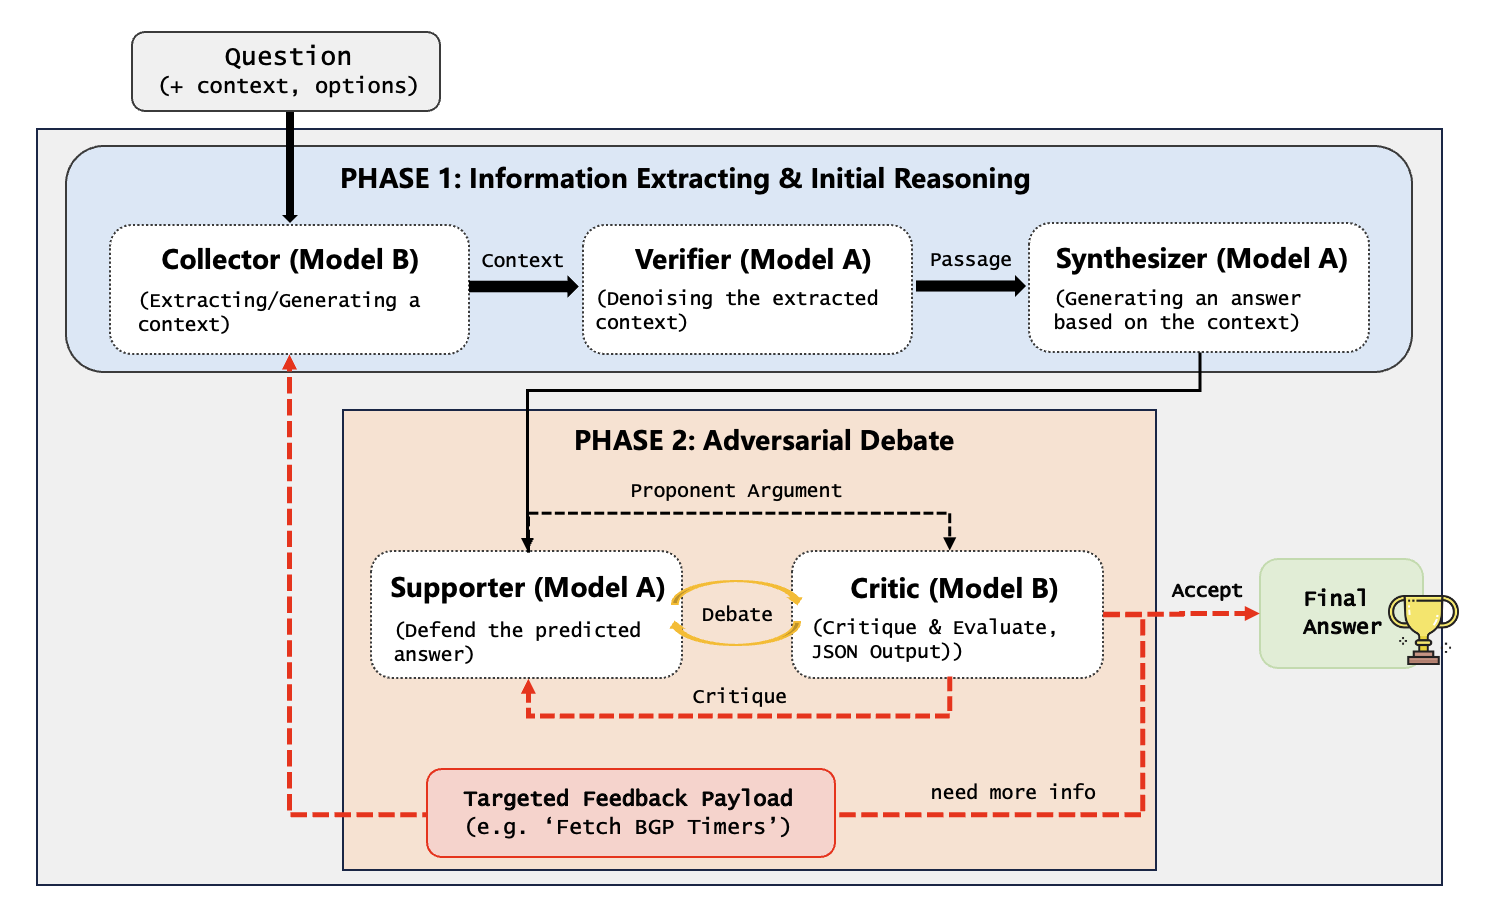
\includegraphics[width=\columnwidth]{figure/multi_agent_arch.png}
%   \caption{Multi-agent debate and hierarchical feedback architecture of NetAgent.}
%   \label{fig:multi_agent_arch}
% \end{figure}

% ============================================================
\subsection{Agent Roles}
% ============================================================

The MAS comprises collector, verifier, synthesizer, proponent and critic.
The \textbf{Collector} extracts relevant configuration blocks from the raw context (or generates context from domain knowledge when none is available) and revises its extraction scope upon Outer Loop re-entry.
The \textbf{Verifier} filters noise from the extracted context to produce a clean passage; for L4/L5 questions requiring full topology reasoning, filtering is bypassed (\textbf{BYPASS}).
The \textbf{Synthesizer} derives a candidate answer from the passage; for L5 fault-analysis questions, it follows a six-step structured inference procedure.
The \textbf{Proponent} constructs a passage-grounded supporting argument and, upon receiving critique, refines the candidate answer via \textit{Self-Refine}~\cite{madaan2023selfrefine}.
The \textbf{Critic} renders one of three verdicts based on passage evidence:

\begin{equation}
\small
  \text{verdict} =
  \begin{cases}
    \textit{ACCEPT}           & \text{if } \text{evidence}(p, a) = \text{True} \\
    \textit{CONTINUE\_DEBATE} & \text{if } \text{evidence}(p, a) = \text{Partial} \\
    \textit{NEED\_MORE\_INFO} & \text{if } \text{evidence}(p, a) = \text{None}
  \end{cases}
\end{equation}

% \begin{table}[!t]
% \centering
% \caption{Summary of NetAgent's five specialized agents.}
% \label{tab:agent_roles}
% \resizebox{1.1\columnwidth}{!}{%
% \begin{tabular}{|l|l|l|}
% \hline
% \textbf{Agent} & \textbf{Role} & \textbf{Output} \\ \hline
% Collector  & Extract relevant config blocks & Extracted Context \\ \hline
% Verifier   & Filter noise; bypass for L4/L5 & Passage \\ \hline
% Synthesizer & Derive candidate answer & Candidate Answer \\ \hline
% Proponent  & Build supporting argument; self-refine & Proponent Argument \\ \hline
% Critic     & Verdict: ACCEPT / CONTINUE / NEED\_INFO & Verdict + Feedback \\ \hline
% \end{tabular}%
% }
% \end{table}

% ============================================================
\subsection{Hierarchical Loop Structure}
% ============================================================

The Critic's verdict drives a two-level feedback loop.
An \textit{ACCEPT} verdict terminates the pipeline and outputs the consensus answer.
A \textit{CONTINUE\_DEBATE} verdict triggers an \textbf{Inner Loop}: the Proponent refines the answer based on the critique and resubmits to the Critic (up to 3 turns).
A \textit{NEED\_MORE\_INFO} verdict triggers an \textbf{Outer Loop}: the Collector re-extracts context guided by the feedback payload and restarts the pipeline (up to 3 iterations).
This structure combines adversarial debate~\cite{du2024improving} and skeptical verification~\cite{liang2024encouraging} to substantially improve factual accuracy in the network configuration domain.



% % ============================================================
% %  NetAgent: Multi-Agent Debate System Based on LangGraph
% % ============================================================

% \section{NetAgent: Multi-Agent Debate System Based on LangGraph}

% This section describes the architecture and implementation of NetAgent, a MAS proposed to improve the reliability and reasoning accuracy of network QA.
% NetAgent is built on the LangGraph framework and, as illustrated in Fig.~\ref{fig:multi_agent_arch}, employs a collaborative architecture in which five specialized agents share state to cooperate across the full pipeline from information extraction to critical verification.
% To address the hallucination and context leakage problems that arise when a single LLM processes large network configuration files at once, NetAgent hierarchically combines an information refinement phase (\textit{Phase~1}) and an adversarial verification phase (\textit{Phase~2}).

% % 본 장에서는 네트워크 QA의 신뢰성과 추론 정확도를 향상시키기 위하여 제안하는 MAS인 NetAgent의 아키텍처 및 구현 내용을 기술한다.
% % NetAgent는 LangGraph 프레임워크를 기반으로 구현되었으며, 그림~\ref{fig:multi_agent_arch}와 같이 정보 추출부터 비판적 검증까지 5개의 특화된 에이전트가 공유 상태를 통해 협업하는 구조를 가진다. 
% % Single LLM이 방대한 네트워크 설정 파일을 한 번에 처리할 때 발생하는 hallucination과 context leakage 문제를 해결하기 위하여, NetAgent는 정보 정제 단계(\textit{Phase 1})와 찬반 검증 단계(\textit{Phase 2})를 계층적으로 결합한다.

% \begin{figure*}[!t]
%     \vspace{-10pt}
%   \centering
%   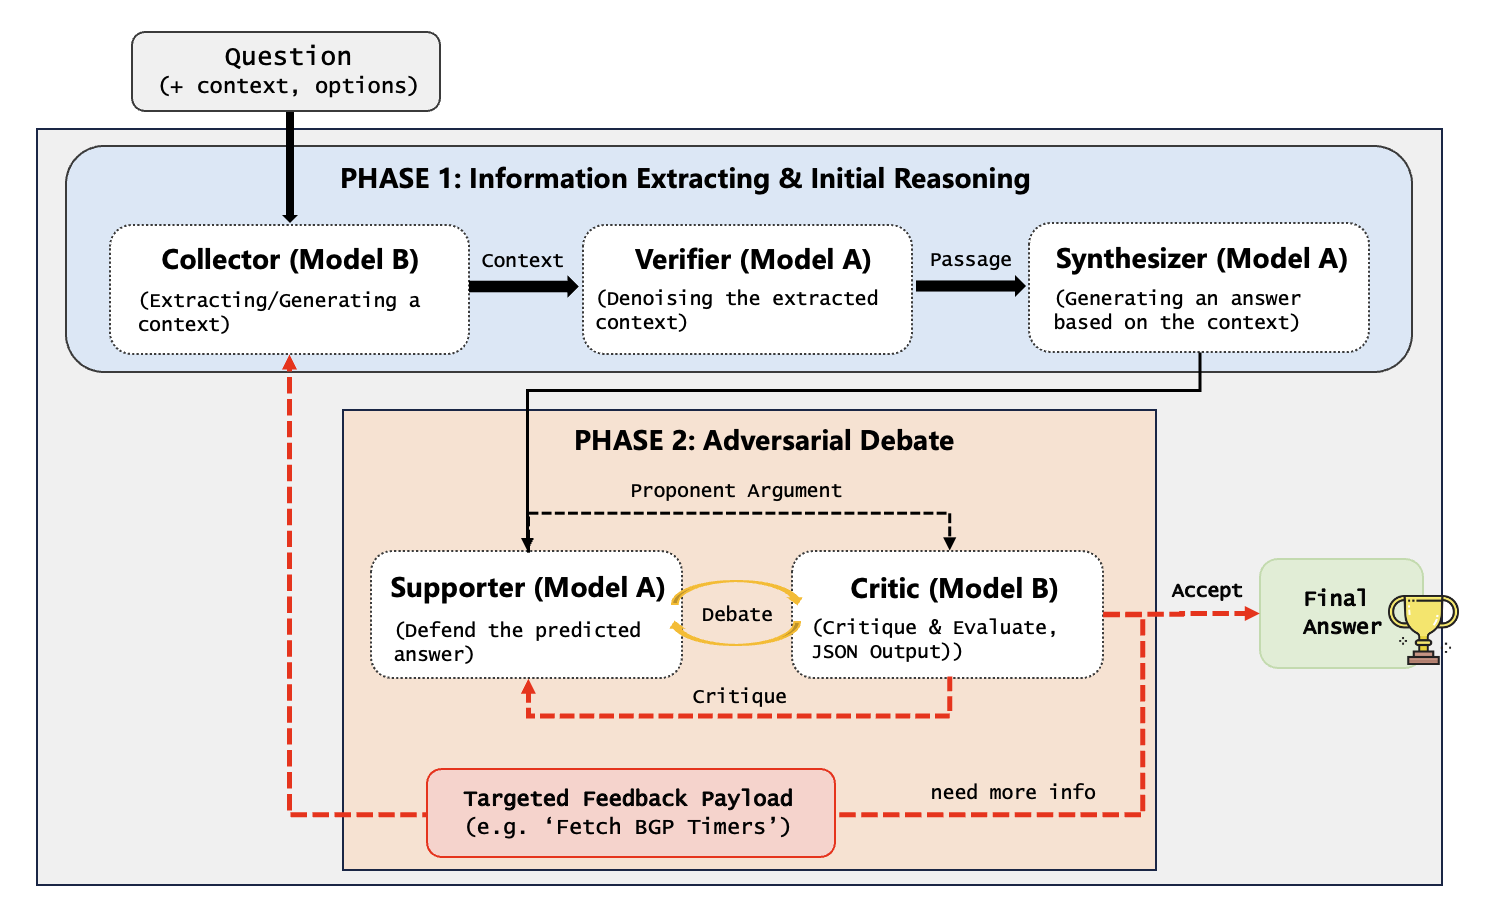
\includegraphics[width=0.7\textwidth]{figure/multi_agent_arch.png}
%   \caption{Multi-agent debate and hierarchical feedback architecture of NetAgent.}
%   \label{fig:multi_agent_arch}
%   \vspace{-10pt}
% \end{figure*}

% % ============================================================
% \subsection{Agent Configuration and Roles}
% % ============================================================

% NetAgent employs a five-agent pipeline, with each agent executing a specialized function to manage the complexity of network domain knowledge.
% % Following X-MAS~\cite{ye2025xmas}, a heterogeneous LLM configuration is adopted: agents requiring language generation capabilities (Verifier, Synthesizer, Proponent) are assigned \textbf{Model~A}, while agents requiring precise logical reasoning (Collector, Critic) are assigned \textbf{Model~B}, thereby leveraging each model's strengths according to its role while maintaining cost efficiency.

% % For Model~A, Gemini-3.1-Flash-Lite is selected based on cost-efficiency considerations~\cite{gemini31_flash_lite_2026}.
% % Given that the multi-agent pipeline invokes numerous LLM calls per query, assigning this model to high-frequency agents (Verifier, Synthesizer, Proponent) reduces overall inference costs while preserving text generation quality.
% % For Model~B, GPT-4o mini is assigned to the Collector and Critic, as the accuracy of information extraction and the logical rigor of verdict judgments directly impact the system's overall performance.
% A hybrid infrastructure supporting both cloud API access (OpenAI API, OpenRouter) and local 4-bit quantized GPU inference ensures operational flexibility. The roles of each agent are as follows.

% % NetAgent는 네트워크 도메인 지식의 복잡성을 해결하기 위하여 세분화된 역할을 수행하는 5개 에이전트 파이프라인으로 구성된다.
% % X-MAS~\cite{ye2025xmas}를 바탕으로 Heterogeneous LLM 구성을 채택하며, 언어 생성 능력이 요구되는 에이전트(Verifier, Synthesizer, Proponent)에는 \textbf{Model A}로, 엄격한 논리 판단이 요구되는 에이전트(Collector, Critic)에는 \textbf{Model B}로 구성하여 각 모델의 강점을 역할에 맞게 특화하면서 비용 효율을 동시에 확보한다.

% % 본 논문에서는 비용 효율성을 생각하여 Model A로 Gemini-3.1-Flash-Lite를 선택하였다~\cite{gemini31_flash_lite_2026}.
% % 다중 에이전트 파이프라인 특성상 단일 질의당 다수의 LLM 호출이 발생하므로, 우리는 호출 빈도가 높은 Verifier, Synthesizer, Proponent에 이 모델을 배치함으로써 전체 추론 비용을 절감하면서도 텍스트 생성 품질을 유지한다. 
% % 반면, 정보 추출의 정밀도(Collector)와 찬반 판정의 논리적 엄밀성(Critic)은 시스템 전체의 정확도에 직접적인 영향을 미치므로, 우리는 두 에이전트들을 Model B로 GPT-4o mini를 배치하여 판단 신뢰성을 확보한다. 또한 우리는 OpenAI API, OpenRouter와 4-bit 양자화된 로컬 GPU 모드를 모두 지원하는 하이브리드 인프라를 통해 운영 유연성을 확보한다.
% % 각 에이전트는 다음과 같은 역할을 수행한다.


% \begin{enumerate}

%   % ---- Agent 1 ---
% \item \textbf{Collector (Information Extractor):}
%   Extracts the \texttt{Extracted Context} most pertinent to the question from the input \texttt{Raw Context}.
%   For the NetConfig dataset, device-specific configuration blocks (\texttt{.cfg}) are identified, and only relevant sections are selectively extracted to enhance information density.
%   In the absence of context (e.g., context-free multiple-choice questions), the agent generates relevant context directly from its domain knowledge.
%   Upon re-entry into the Outer Loop, the extraction scope is adjusted to incorporate the Feedback Payload provided by the Critic.
%     %   % ---- Agent 1 ----
% %   \item \textbf{Collector (Information Extractor) --- Model B:}
% %     입력된 \texttt{Raw Context}로부터 질문과 직결된
% %     \texttt{Extracted context}를 추출한다.
% %     NetConfig 데이터셋의 경우, 장비별 설정 블록(\texttt{.cfg})을 식별하여 관련 섹션을 위주로 추출함으로써 정보 밀도를 높인다.
% %     컨텍스트가 존재하지 않는 경우(예: 컨텍스트 없는 Multiple-choice 문제)에는 에이전트 자체의 도메인 지식을 기반으로 질문 및 선택지와 관련된 컨텍스트를 직접 생성한다.
% %     Outer Loop 재진입 시에는 Critic이 전달한 피드백 페이로드(Feedback Payload)를 반영하여 추출 범위를 재조정한다.

% % ---- Agent 2 ----
% \item \textbf{Verifier (Passage Generator):}
%   Eliminates noise unrelated to the question from the \texttt{Extracted Context} and generates a \texttt{Passage} containing only the essential information.
%   To preserve the fidelity of the original text, relevant lines are selectively retained rather than arbitrarily summarized or altered.
%   The \textit{``When in doubt, keep the line''} principle is employed to prevent the inadvertent removal of answer-bearing lines during aggressive filtering.
%   For path-tracing (L4) and fault-analysis (L5) questions, however, the full context is required to support complex cross-referencing; in these cases, filtering is bypassed (\textbf{BYPASS}) and the \texttt{Extracted Context} is directly passed as the \texttt{Passage}.

% %   % ---- Agent 2 ----
% %   \item \textbf{Verifier (Passage Generator) --- Model A:}
% %     \texttt{extracted\_context}에서 질문과 무관한 노이즈를 제거하여 필요한 정보들로만 이루어진 \texttt{Passage}로 정리한다.
% %     원본 텍스트의 정합성을 유지하기 위하여 임의의 요약이나 수정 대신 관련 라인을 선택적으로 보존하는 방식을 채택한다.
% %     이때 \textit{"의심스러우면 보존(When in doubt, keep the line)"} 원칙을 적용하여 공격적 필터링으로 인한 정답 라인 소실을 방지한다.
% %     단, 경로 추적(L4) 및 장애 분석(L5) 수준의 질문에 대해서는 복잡한 교차 추론에 필요한 전체 컨텍스트가 보존되어야 하므로 필터링을 우회(\textbf{BYPASS})하고, \texttt{extracted\_context}를 그대로 \texttt{Passage}로 전달한다.



% % ---- Agent 3 ----
% \item \textbf{Synthesizer (Answer Deriver):}
%   Generates an initial hypothesis and candidate answer from the refined \texttt{Passage}.
%   Output formats optimized for each dataset type (Descriptive, Multiple-choice, Short Answer, etc.) are applied to ensure readability and consistency for the subsequent debate phase.
%   For L5 (fault analysis) questions, which require complex reasoning across the entire topology, the agent explicitly performs the following six-step structured inference:
%   \begin{enumerate}
%     \item Construct normal topology --- enumerate all device interfaces and routing tables.
%     \item Trace normal path --- verify the source$\rightarrow$destination path hop-by-hop.
%     \item Apply fault --- remove the designated link or device and mark affected interfaces and routes.
%     \item Re-trace post-fault path --- identify NO\_ROUTE points or alternative paths.
%     \item Determine answer --- classify as Blocking device, Possible, Impossible, or Count.
%     \item Produce final output --- format the result according to the specified \texttt{answer\_type}.
%   \end{enumerate}

% %   % ---- Agent 3 ----
% %   \item \textbf{Synthesizer (Answer Deriver) --- Model A:}
% %     정제된 패시지를 바탕으로 초기 가설 및 후보 답변(Candidate Answer)을 생성한다.
% %     데이터셋 타입(Descriptive, Multiple-choice, Short Answer 등)에 최적화된 출력 형식을 적용하여 후속 토론의 가독성을 보장한다.
% %     특히 L5(장애 분석) 질문의 경우, 전체 토폴로지에 대한 복합 추론이 요구되므로 아래 6단계 구조화 추론을 명시적으로 수행하도록 설계한다.
% %     \begin{enumerate}
% %       \item 정상 토폴로지 구축 --- 모든 장비의 인터페이스 및 라우팅 테이블 나열
% %       \item 정상 경로 추적 --- hop-by-hop으로 src$\rightarrow$dst 경로 확인
% %       \item 장애 적용 --- 지정된 링크/장비 제거 후 영향받는 인터페이스·라우트 표시
% %       \item 장애 후 경로 재추적 --- NO\_ROUTE 지점 또는 대안 경로 탐색
% %       \item 답 결정 --- Blocking device / Possible / Impossible / Count 결정
% %       \item 최종 한 줄 출력 --- 규정된 \texttt{answer\_type} 형식으로 출력
% %     \end{enumerate}

%   % ---- Agent 4 ----
% % ---- Agent 4 ----
% \item \textbf{Proponent (Supporter):}
%   Receives the candidate answer generated by the Synthesizer and constructs a passage-grounded supporting argument, which is then forwarded to the Critic.
%   This process leverages the CAMEL~\cite{li2023camel} collaborative framework to present evidence that justifies the answer.
%   Upon receiving a \textit{CONTINUE\_DEBATE} verdict and accompanying critique from the Critic, the Proponent generates a counter-argument grounded in the passage, refines the candidate answer, and re-submits it to the Critic, thereby implementing \textit{Self-Refine}~\cite{madaan2023selfrefine} within the multi-agent pipeline.

% %   % ---- Agent 4 ----
% %   \item \textbf{Proponent (Supporter) --- Model A:}
% %     Synthesizer가 생성한 후보 답변을 입력받아 패시지에 근거한 candidate answer의 옹호 논거를 구성하고, 이를 Critic에게 전달한다.
% %     이 과정은 CAMEL~\cite{li2023camel} 협업 모델을 적용한 것으로, 답변의 정당성을 뒷받침하는 근거를 제시한다.
% %     이후 Critic으로부터 \textit{CONTINUE\_DEBATE} 판정과 함께 비판을 수신하면,
% %     패시지에 근거한 반론을 구성하여 답변을 정교화한 뒤 다시 Critic에게 전달한다\textit{Self-Refine}~\cite{madaan2023selfrefine}.


% % ---- Agent 5 ----
% \item \textbf{Critic (Skeptic):}
%   Serves as the system’s final verifier by evaluating the appropriateness of the candidate answer through synthesis of the passage and the Proponent’s supporting argument.
%   A verdict is issued according to the three criteria:
%   \begin{itemize}
%     \item \textit{ACCEPT}: When clear evidence supporting the candidate answer is present in the passage, the process terminates and the final consensus answer is output.
%     \item \textit{CONTINUE\_DEBATE}: When evidence exists but the candidate answer is inconsistent with it or contains logical gaps, evidence-backed criticism is forwarded to the Proponent to initiate an Inner Loop.
%     \item \textit{NEED\_MORE\_INFO}: When the passage contains irrelevant content or lacks refutable relevant evidence, a feedback payload specifying the missing information is generated and sent to the Collector to initiate an Outer Loop.
%   \end{itemize}

% % \begin{equation}
% % \small
% %   \text{verdict} =
% %   \begin{cases}
% %     \textit{ACCEPT}           & \text{if } \text{evidence}(p, a) = \text{True} \\
% %     \textit{CONTINUE\_DEBATE} & \text{if } \text{evidence}(p, a) = \text{Partial} \\
% %     \textit{NEED\_MORE\_INFO} & \text{if } \text{evidence}(p, a) = \text{None}
% %   \end{cases}
% % \end{equation}
% %   % ---- Agent 5 ----
% %   \item \textbf{Critic (Skeptic) --- Model B:}
% %     시스템의 최종 검증자로서, 패시지와 옹호 의견을 종합하여 후보 답변의 적절성을 평가한다.
% %     표~\ref{tab:critic_status}에 제시된 세 가지 기준에 따라 최종 수용 여부를 판정하며, 구체적인 판정 조건은 다음과 같다.
% %     \begin{itemize}
% %       \item \textit{ACCEPT}: 패시지에서 후보 답변에 대한 명백한 근거를 확인할 수 있을 때,
% %             프로세스를 종료하고 최종 합의 답변(Consensus Answer)을 출력한다.
% %       \item \textit{CONTINUE\_DEBATE}: 패시지에 근거는 존재하나 후보 답변이 이와 일치하지 않거나
% %             논리적 비약이 있을 때, 근거를 제시한 비판을 Proponent에게 전달하여
% %             Inner Loop(내부 토론)을 기동한다.
% %       \item \textit{NEED\_MORE\_INFO}: 패시지에 질문과 무관한 내용이 포함되어 있거나
% %             반박 가능한 관련 근거가 존재하지 않을 때,
% %             부족한 정보를 명시한 피드백 페이로드를 생성하여 Collector에게 전달하고
% %             Outer Loop(외부 재추출)을 기동한다.
% %     \end{itemize}

% \end{enumerate}

% % \begin{enumerate}





% % \end{enumerate}

% % ============================================================
% \subsection{Full Pipeline and Hierarchical Loop Structure}
% % ============================================================

% The NetAgent pipeline consists of two debate phases connected by a hierarchical feedback loop.
% Algorithm~\ref{alg:netagent} formalizes the overall flow; the processing steps and branching conditions of each phase are described below.

% \subsubsection{Phase 1: Information Retrieval and Initial Reasoning}

% This phase executes as a sequential pipeline in which agents process raw materials for reasoning and derive a candidate answer.

% \begin{enumerate}
%   \item \textbf{Collector}: Analyzes the input question and either extracts relevant configuration blocks from the Raw Context or, when no context is available, generates one from domain knowledge.
%         Upon Outer Loop re-entry, the extraction scope is revised to incorporate the feedback generated by the Critic.

%   \item \textbf{Verifier}: Assesses the difficulty level of the question and determines the branching strategy.
%         \begin{itemize}
%           \item L1/L2/L3 (single-device fact extraction and multi-device comparison):
%                 Filtering is applied to produce a high-quality passage.
%           \item L4/L5 (path tracing and fault analysis):
%                 Since the overall configuration must be examined, filtering is bypassed and the \texttt{Extracted Context} is passed directly as the passage.
%         \end{itemize}

%   \item \textbf{Synthesizer}: Receives the passage as input and derives an initial candidate answer based on the \textit{Generate-then-Read}~\cite{yu2023generate} strategy.
%         For L5 questions, the six-step Fault Analysis reasoning described above is performed.
% \end{enumerate}

% % NetAgent의 파이프라인은 두 개의 Debate 단계와 이를 연결하는 계층적 피드백 루프로 구성된다.
% % 알고리즘~\ref{alg:netagent}은 전체 흐름을 형식화하여 정리한 것이며, 각 단계의 처리 과정과 분기 조건은 다음과 같다.

% % \subsubsection{Phase 1: 정보 검색 및 초기 추론 (Debate 1)}

% % 이 단계는 순차적 파이프라인으로 수행되며, 에이전트들은 추론의 원재료를 가공하여 후보 답변을 도출하는 작업을 수행한다.

% % \begin{enumerate}
% %   \item \textbf{Collector}: 입력 질문을 분석하여 Raw Context에서
% %         관련 설정 블록을 추출하거나, 컨텍스트가 없는 경우 도메인 지식으로 생성한다.
% %         Outer Loop 재진입 시에는 Critic이 생성한 피드백을 반영하여
% %         추출 범위를 수정한 뒤 재수행한다.

% %   \item \textbf{Verifier}: 추출된 컨텍스트에 대해 질문 난이도 수준을 판단하여 분기를 결정한다.
% %         \begin{itemize}
% %           \item L1/L2/L3 (단일 장비 사실 추출 및 다중 장비 비교):
% %                 필터링을 적용하여 패시지를 생성한다.
% %           \item L4/L5 (경로 추적 및 장애 분석): 전반적인 설정을 확인해야하므로 필터링을 우회(BYPASS)하고 \texttt{extracted\_context}를
% %                 그대로 패시지로 전달한다.
% %         \end{itemize}

% %   \item \textbf{Synthesizer}: 패시지를 입력으로 받아
% %         \textit{Generate-then-Read}~\cite{yu2023generate} 전략을 기반으로
% %         초기 후보 답변을 도출한다.
% %         L5 질문의 경우 앞서 기술한 6단계 Fault Analysis 추론을 수행한다.
% % \end{enumerate}


% \subsubsection{Phase 2: Hierarchical Adversarial Debate}

% In the second phase, the reliability of the candidate answer is verified through multi-agent interaction.
% The candidate answer generated by the Synthesizer is first forwarded to the Proponent, where a supporting argument is constructed; the Critic then synthesizes the passage and the argument to render a verdict.
% Depending on the Critic's verdict, one of the following three branches is activated.

% % 두 번째 단계에서는 다중 에이전트 상호작용을 통해 후보 답변의 신뢰성을 검증한다.
% % Synthesizer가 생성한 후보 답변은 먼저 Proponent에게 전달되어 옹호 논거가 구성되며,
% % 이후 Critic이 패시지와 옹호 논거를 종합하여 판정을 내린다.
% % Critic의 판정 상태(table~\ref{tab:critic_status})에 따라 아래 세 가지 분기 중 하나가 활성화된다.


% \begin{itemize}
%   \item \textbf{Termination (\textit{ACCEPT}):}
%     When the Critic identifies clear evidence in the passage, \textit{ACCEPT} is returned, the final consensus answer is output, and the process terminates.

%   \item \textbf{Inner Loop --- \textit{CONTINUE\_DEBATE}:}
%     When the Critic detects a logical leap, feedback containing the critique is forwarded to the Proponent.
%     The Proponent presents a passage-grounded counter-argument, refines the answer, and re-submits the updated Proponent Argument to the Critic.
%     This process repeats while \texttt{inner\_turn\_count} $<=$ 3; upon reaching the limit, the current candidate answer is finalized and the system terminates.

%   \item \textbf{Outer Loop --- \textit{NEED\_MORE\_INFO}:}
%     When the Critic determines that the current passage lacks necessary information, a feedback payload specifying what information is required is generated and the Collector is re-invoked.
%     The Collector revises the extraction scope based on the feedback and re-executes the pipeline.
%     Upon reaching \texttt{outer\_loop\_count} $\geq$ 3, the current candidate answer is finalized and the system is forcibly terminated.

% %   \item \textbf{정상 종료 (\textit{ACCEPT}):}
% %     Critic이 패시지에서 명백한 근거를 확인하면 \textit{ACCEPT}를 반환하고,
% %     최종 합의 답변을 출력하며 프로세스를 종료한다.

% %   \item \textbf{Inner Loop --- \textit{CONTINUE\_DEBATE}:}
% %     Critic이 논리적 비약을 감지하면 비판(Critique)을 포함한 피드백을 Proponent에게 전달한다.
% %     Proponent는 패시지에 근거한 반론을 제시하고 답변을 정교화한 뒤,
% %     갱신된 Proponent Argument를 다시 Critic에게 전달한다.
% %     이 과정은 \texttt{inner\_turn\_count} $<$ 3인 동안 반복되며,
% %     상한에 도달하면 현재 후보 답변을 최종 답변으로 확정하여 시스템이 종료된다.

% %   \item \textbf{Outer Loop --- \textit{NEED\_MORE\_INFO}:}
% %     Critic이 현재 패시지에 필요한 정보가 부족하다고 판단하면,
% %     어떤 정보가 필요한지를 명시한 피드백 페이로드를 생성하여
% %     Phase 1의 Collector을 재실행한다.
% %     Collector는 피드백을 반영하여 추출 범위를 수정하고 파이프라인을 재수행한다.
% %     \texttt{outer\_loop\_count} $\geq$ 3에 도달하면 현재 후보 답변을
% %     최종 답변으로 확정하여 강제 종료한다.

% \end{itemize}

% This hierarchical structure is designed to overcome the limitations of single-model \textit{Self-Refine}~\cite{madaan2023selfrefine}.
% Through adversarial debate~\cite{du2024improving} and skeptical verification~\cite{liang2024encouraging} among multiple agents, factual accuracy in the network configuration domain is substantially improved.

% % 이러한 계층적 구조는 단일 모델의 \textit{Self-Refine}~\cite{madaan2023selfrefine} 한계를 극복하기 위하여 설계되었다. 다중 에이전트 간의 찬반 토론~\cite{du2024improving} 및 회의론적 검증~\cite{liang2024encouraging}을 통해 네트워크 설정 도메인에서의 사실성(Factuality)을 향상시킨다.


